\documentclass[11pt]{article}
\usepackage[margin=0.85in]{geometry}
\usepackage{amsmath,amssymb,graphicx,booktabs}
\setlength{\parindent}{0pt}
\setlength{\parskip}{5pt}
\begin{document}
\begin{center}
{\Large Project 1: Double-descent experiment}\\[4pt]
00103335: Deep Learning and Reinforcement Learning --- Fall 2026
\end{center}

\textbf{Method (a), (c).}
For each $s\in\{5,2,1\}$, set $\beta=\sqrt{s}\,e_1$, $n=200$, and use
\[
 p\in\{20,40,60,80,100,120,140,160,180,199,200,220,240,260,300,400,600\}.
\]
For every $(s,p)$, perform 20 independent repetitions. In each repetition,
draw fresh, mutually independent $X\in\mathbb R^{200\times p}$,
$\varepsilon\in\mathbb R^{200}$, and $X_{\rm test}\in\mathbb R^{2000\times p}$
with independent standard Gaussian entries. Form $y=X\beta+\varepsilon$,
compute the minimum-norm solution $\widehat\beta=X^+y$ using
\texttt{numpy.linalg.lstsq}, and record
\[
 R=\frac1{2000}\|X_{\rm test}(\widehat\beta-\beta)\|_2^2.
\]
The test target is noiseless, as specified. The random seed is 20260914;
\texttt{results/risks.csv} contains all 1,020 risks.

\textbf{Peaks (b), (c).}
Each plot below uses the 20 recorded risks at each $p$. The vertical axis
is logarithmic; medians and arithmetic sample means are computed on the
original risk scale. Their observed maxima are:
\begin{center}
\begin{tabular}{crrrr}
\toprule
$\beta$ & Median peak $p$ & Median risk & Mean peak $p$ & Mean risk\\
\midrule
$\sqrt5\,e_1$ & 200 & 433.826 & 200 & 93888.507\\
$\sqrt2\,e_1$ & 199 & 177.463 & 200 & 1149.604\\
$e_1$        & 200 & 448.124 & 200 & 5586.063\\
\bottomrule
\end{tabular}
\end{center}
Risk rises sharply near the interpolation threshold $p=n=200$ and
falls on the overparameterized side. For $\beta=\sqrt2\,e_1$, the
observed median peaks at $199$, slightly above the median $170.975$ at
$200$. These are finite-sample peaks from 20 repetitions.
The much larger mean than median near the threshold reflects extreme
risks in some repetitions.

\textbf{(b) $\beta=\sqrt5\,e_1$.}
\begin{center}
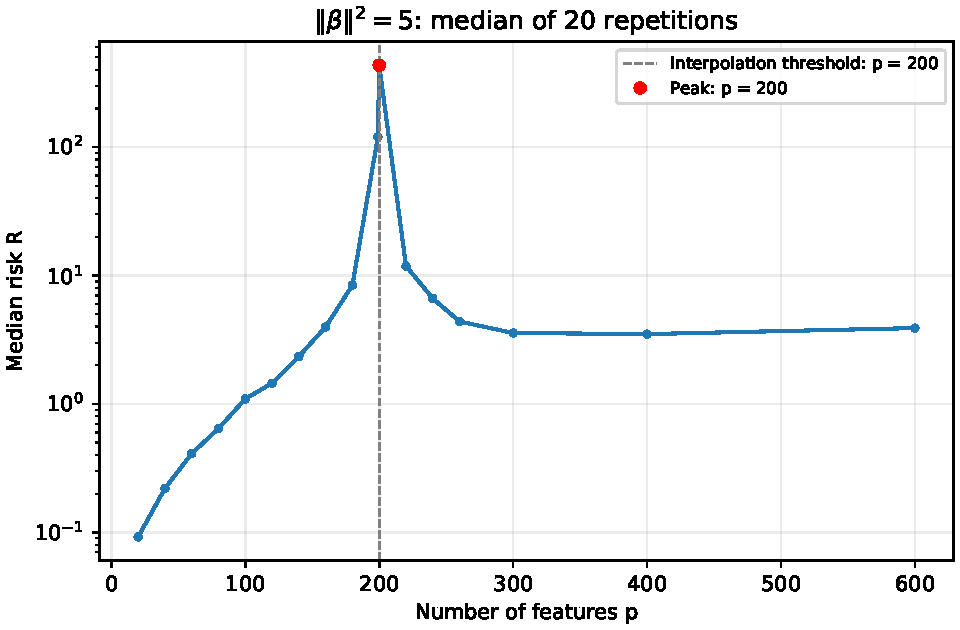
\includegraphics[width=0.49\linewidth]{results/signal_5_median.pdf}\hfill
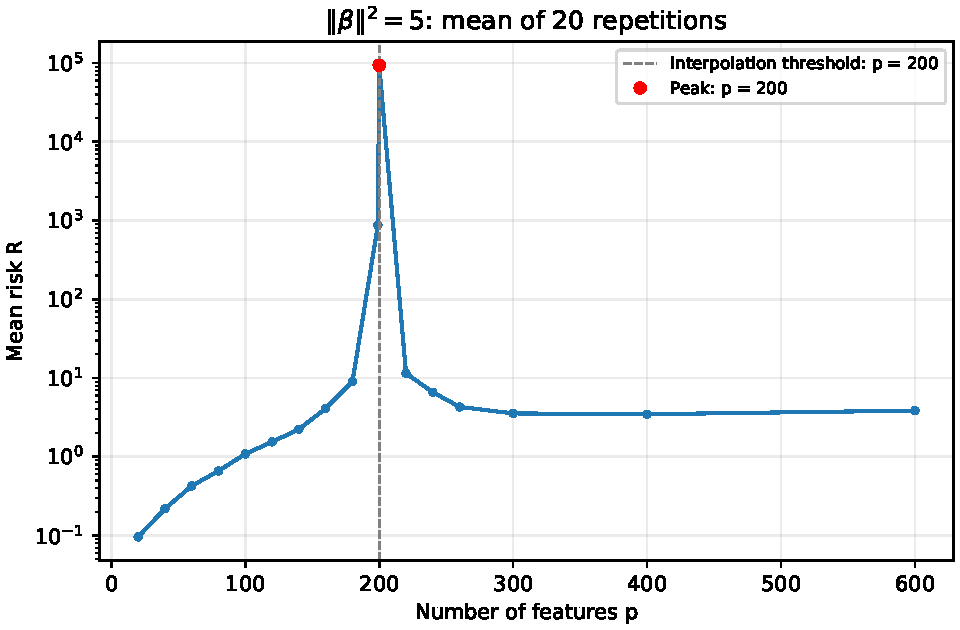
\includegraphics[width=0.49\linewidth]{results/signal_5_mean.pdf}
\end{center}

\newpage
\textbf{(c) $\beta=\sqrt2\,e_1$.}
\begin{center}
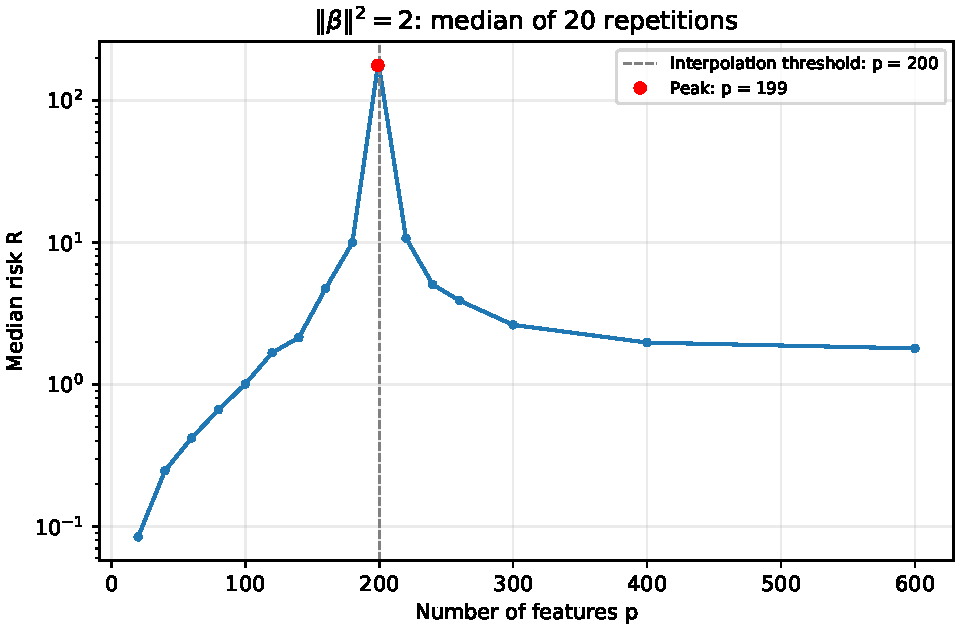
\includegraphics[width=0.49\linewidth]{results/signal_2_median.pdf}\hfill
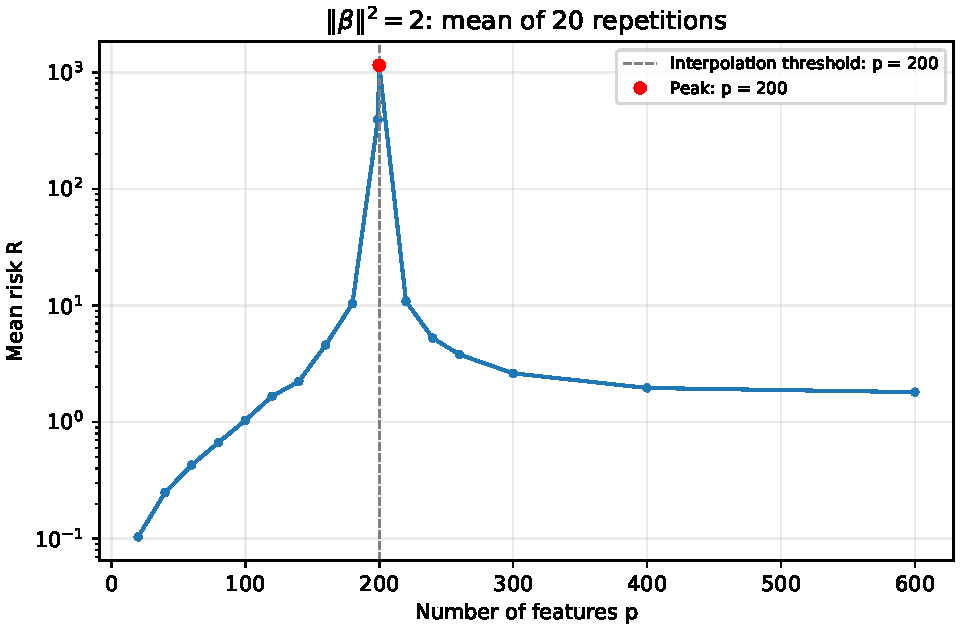
\includegraphics[width=0.49\linewidth]{results/signal_2_mean.pdf}
\end{center}

\textbf{(c) $\beta=e_1$.}
\begin{center}
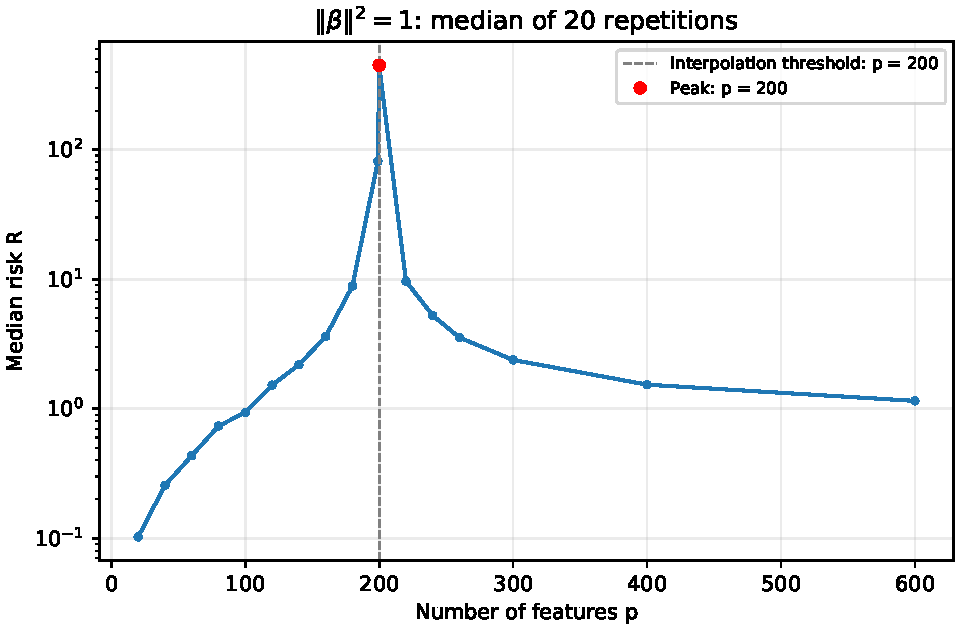
\includegraphics[width=0.49\linewidth]{results/signal_1_median.pdf}\hfill
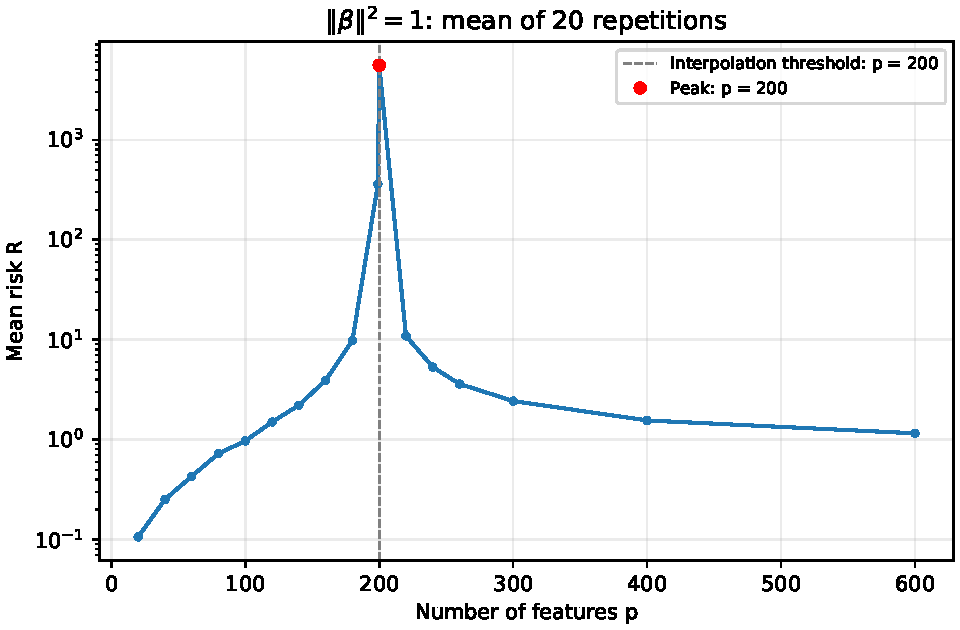
\includegraphics[width=0.49\linewidth]{results/signal_1_mean.pdf}
\end{center}
\end{document}
